\documentclass[11pt, bibliography=totocnumbered]{scrartcl}
\usepackage[ngerman]{babel}
\usepackage{placeins}
\usepackage{mathtools}
\title{Dokumentation - Projekt Kreuzgew\"olbe}
\author{Java-Gruppe 2 (Dieter Dirk J\"uptner, Sascha Knapp, Kai Liu, Paul S\"oldner)}

\setlength{\parindent}{0pt}
\setlength{\parskip}{\baselineskip}
\usepackage{graphicx}
\usepackage{listings}
\usepackage{color}
\usepackage{amsmath}
\usepackage{bm}
\definecolor{dkgreen}{rgb}{0,0.6,0}
\definecolor{gray}{rgb}{0.5,0.5,0.5}
\definecolor{mauve}{rgb}{0.58,0,0.82}

\lstset{frame=tb,
	language=Java,
	aboveskip=3mm,
	belowskip=3mm,
	showstringspaces=false,
	columns=flexible,
	basicstyle={\small\ttfamily},
	numbers=none,
	numberstyle=\tiny\color{gray},
	keywordstyle=\color{blue},
	commentstyle=\color{dkgreen},
	stringstyle=\color{mauve},
	breaklines=true,
	breakatwhitespace=true,
	tabsize=3
}

\begin{document}
	\begin{titlepage}
		\begin{center}
			\vspace*{2cm}
			
			\huge
			\textbf{Approximation eines Kreuzgew\"olbes anhand von Messpunkten und Berechnung von dessen Oberfl\"ache}
			
			\vspace{1.5cm}
			\LARGE
			Dokumentation zur F\"acher\"ubergreifenden Projektarbeit
		\end{center}    
		\vspace{1cm}
		
		\vfill{}
		\large
		\begin{tabular}{@{}l l}
			Eingereicht von: & \\
			Sascha Knapp \\
			Paul S\"oldner \\
			\\
			Datum: \today \\
			\\
		\end{tabular}
		\vfill
	\end{titlepage}
\newpage
\tableofcontents
\newpage
\section{Klassendiagramm}
\includegraphics[width=1.2\textwidth]{C:/Users/user/Desktop/uml.png}
\section{Input}
Zum Einlesen der Punkte aus einer Textdatei, werden die x-, y- und z-Werte der Punkte zeilenweise in der Datei gespeichert und jeweils mit einem Leerzeichen getrennt. Die Punkte k\"onnen dabei unsortiert an das Programm \"ubergeben werden. 
\begin{lstlisting}[caption={Input-Datei}, label={lst:label}, language=Java] 
x_1 y_1 z_1
x_2 y_2 z_2
...
\end{lstlisting}
Die Datei wird mit Hilfe eines FileReaders und BufferedReaders eingelesen. Die einzelnen Zeilen werden an Leerzeichen und Tabulatoren getrennt und als Punkt-Objekte einer ArrayList hinzugef\"ugt.
\begin{lstlisting}[caption={Input-Quellcode}, label={lst:label}, language=Java]
public static ArrayList<ArrayList<Point3D>> orderedReadFromFile(String file) throws IOException {
		FileReader fr = new FileReader(file);
		BufferedReader br = new BufferedReader(fr);

		String zeile = "";
		int zeilennummer = 0;
		ArrayList<ArrayList<Point3D>> ergebnis = new ArrayList<ArrayList<Point3D>>();
		ArrayList<Point3D> liste;
		Point3D p;
		while ((zeile = br.readLine()) != null) {
			if (zeile.isEmpty())
				continue;
			String[] split = zeile.split("\\s+");
			liste = new ArrayList<Point3D>();
			for (int i = 0; i < split.length; i += 3) {

				p = new Point3D(Double.parseDouble(split[i]), Double.parseDouble(split[i + 1]),
						Double.parseDouble(split[i + 2]));
				// p.getPunkt();
				liste.add(p);
			}
			ergebnis.add(zeilennummer, liste);
			zeilennummer++;
		}

		br.close();

		System.out.println("File '" + file + "' wurde erfolgreich eingelesen.");

		return ergebnis;
	}
\end{lstlisting}
\section{Testdaten - Erzeugung}

Um Testdaten zu erzeugen haben wir uns eine konkrete Funktion gesucht. Diese wird in der Klasse \glqq{GenerateTest}\grqq benutzt. 

\begin{lstlisting}[caption={Funktion zur Testdaten-Erzeugung}, label={lst:label}, language=Java]
public static double f1(double x, double y) {
	double z = 100 - x*x - y*y;
	return z;
}
\end{lstlisting}

Die Funktion wird in einem Bereich x und y betrachtet. Diese Bereiche werden jeweils in flachen Feldern gespeichert. Die z-Werte der Funktion an den jeweiligen x und y werden in einem 2-Dimensionalen Feld gespeichert.
Die gef\"ullten Felder werden an die \glqq{Output}\grqq - Klasse gegeben, die Punkte getrennt von Abs\"atzen in ein Textdokument schreibt.

\section{Approximation - Regressionspolynome}
Die Klasse \glqq{PolynomialPool}{\grqq } stellt Methoden zum Berechnen der ersten Polynome anhand der gemessenen Punkte zur Verf\"ugung. Dabei werden alle in einer Reihe liegenden Punkte in eine ArrayList gegeben und an die Klasse \glqq{Regression}\grqq  gegeben. Hier wird auch angegeben, welchen Grad die Polynome haben sollen. Wir haben eine Konstante mit dem Wert von 2 Grad gew\"ahlt.


\begin{lstlisting}[caption={Polynome mit x als Raumkoordinate}, label={lst:label}, language=Java]
private void approximateXPolynomials(PointMatrix points) //wenn noch keine Stützpunkte vorhanden sind
{
	for(int i = 0; i < points.stepsInXDirection(); i++)
	{
		Regression r = new Regression();
		ArrayList<Point2D> p = extractPointsInLine_XDirectrion(points, i);
		Polynomial polynomial = r.approximate(p, kDegree);
		polynomial.setRoomCoordinate(data.pm.getPoint(i, 0).getX());
		data.xPolynomials.add(polynomial);
	}
}
\end{lstlisting}

\section{Berechnung der Oberfl\"ache}
Ein einzelnes Fl\"achenst\"uck ergibt sich aus $|\overrightarrow{\boldsymbol{r_u}} \times \overrightarrow{\boldsymbol{r_v}}| \Delta u \Delta v$ \\
Die folgende Methode berechnet dies nun f\"ur jedes Polynom und iteriert \"uber die St\"utzpunkte, um die entsprechenden Funktionswerte $z$ f\"ur $x$ und $y$ auszurechnen. Dabei wird in der Methode die Kr\"ummung an den Stellen au{\ss}er Acht gelassen. \newpage
\begin{lstlisting}[caption={}, label={lst:label}, language=Java]
    public double calcSurfaceArea(ArrayList<Polynomial> funcX, ArrayList<Polynomial> funcY)
    {
        Double result = 0.0;
        for(int i = 0; i < funcX.size()-1; i++)
        {
            for(int j = 0; j < funcY.size()-1; j++)
            {
                Polynomial currFuncX = funcX.get(i);
                Polynomial nextFuncX = funcX.get(i+1);
                Polynomial currFuncY = funcY.get(j);
                Polynomial nextFuncY = funcY.get(j+1);
                Point3D px1 = new Point3D(currFuncX.getRoomCoordinate(), currFuncY.getRoomCoordinate(), currFuncX.derivation(currFuncY.getRoomCoordinate()));
                Point3D py1 = new Point3D(currFuncX.getRoomCoordinate(), currFuncY.getRoomCoordinate(), currFuncY.derivation(currFuncX.getRoomCoordinate()));
                Point3D px2 = new Point3D(nextFuncX.getRoomCoordinate(), currFuncY.getRoomCoordinate(), nextFuncX.derivation(currFuncY.getRoomCoordinate()));
                Point3D py2 = new Point3D(currFuncX.getRoomCoordinate(), nextFuncY.getRoomCoordinate(), nextFuncY.derivation(currFuncX.getRoomCoordinate()));

                Double xDelta = px2.getX()-px1.getX();
                Double yDelta = py2.getY()-py1.getY();

                Vector rx = new Vector(px2.getX()-px1.getX(), px2.getY()-px1.getY(), px2.getZ()-px1.getZ());
                Vector ry = new Vector(py2.getX()-py1.getX(), py2.getY()-py1.getY(), py2.getZ()-py1.getZ());

                Vector crossProduct = new Vector(rx.y() * ry.z()-rx.z()*ry.y(),rx.z()*ry.x()-rx.x()*ry.z(), rx.x()*ry.y()-rx.y()*ry.x());
                Double sum = crossProduct.sum()*xDelta*yDelta;
                result += sum;
            }
        }
        System.out.println("Oberfläche: " + result + " FE");
        return result;
    }
\end{lstlisting}
\section{Benutzeroberfl\"ache}
\hspace*{1cm}
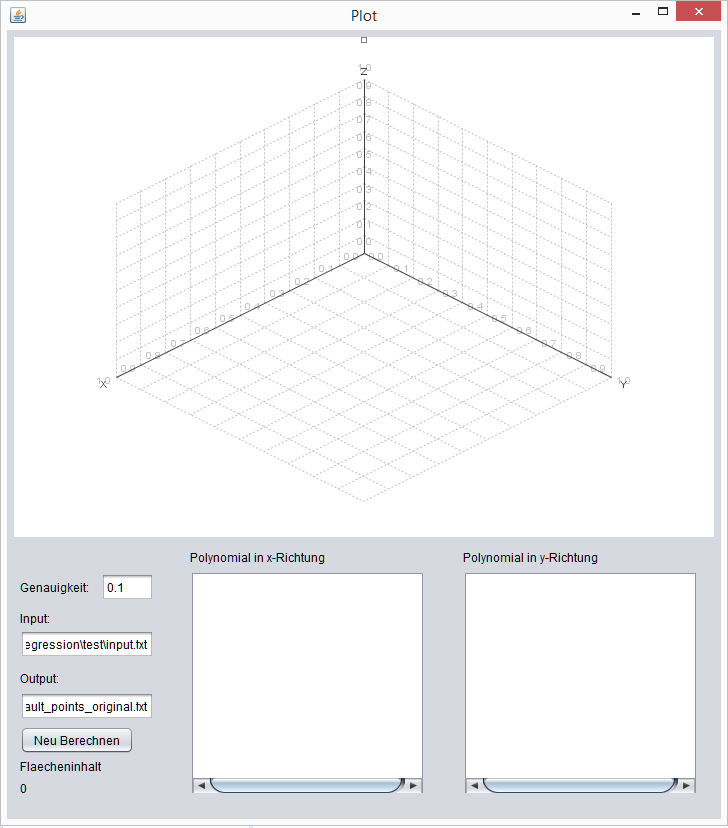
\includegraphics[width=0.8\textwidth]{C:/Users/user/Desktop/Oberflaeche_Standard.png}
\newline
Die Benutzeroberfl\"ache wurde mit Hilfe des Tools \glqq{JMathPlot}{\grqq } erstellt, die dem Benutzer nach dem Einlesen der Eingabedatei direkt den dazugeh\"origen Plot anzeigt. \\ 
Es k\"onnen die Pfade zu der Eingabe- bzw. Ausgabedatei und die Genauigkeit eingeben werden. Die Genauigkeit bestimmt, wie viele Extrapunkte zwischen den eingegeben berechnet werden. \\
Diese Eingaben werden an den \glqq{Controller}{\grqq } weitergegeben, der ggf. weitere Punkte und anschlie{\ss}end die Fl\"ache berechnen l\"asst. Am Ende wird dem Benutzer auf der GUI der Oberfl\"acheninhalt angezeigt. 

\section{Beispiel}
Werden perfekte Punkte (in x- und y-Richtung auf einer Linie) an das Programm \"ubergeben, wird der Plot korrekt angezeigt und eine n\"aherungsweise korrekte Oberfl\"ache berechnet. \\
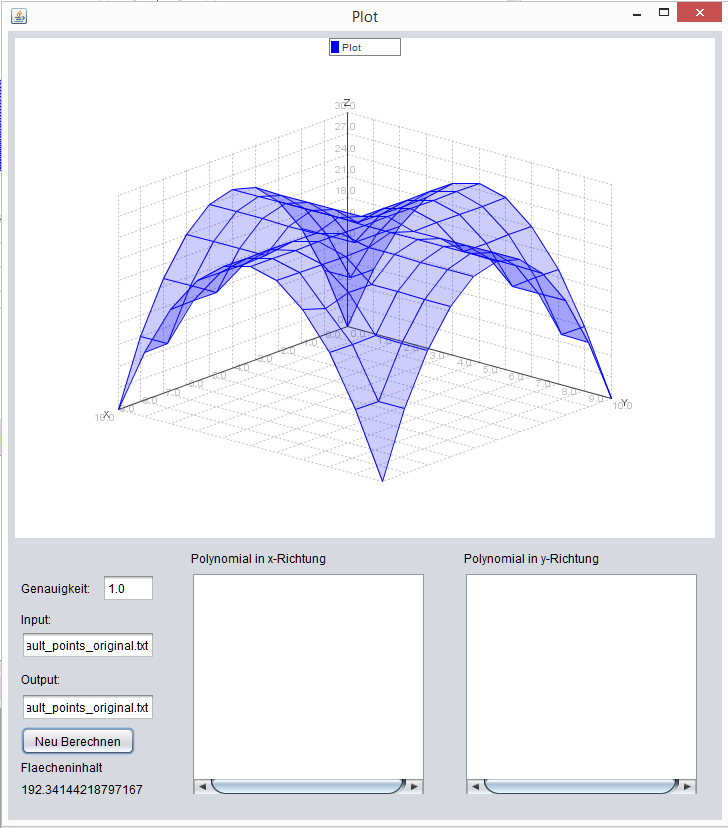
\includegraphics[width=0.8\textwidth]{C:/Users/user/Desktop/oberflaeche_perfekt.png}
\section{Quellen}
\begin{itemize}
\item JMathPlot - https://github.com/yannrichet/jmathplot
\end{itemize}

\section{Ausblick}
\subsection{Echte Punkte}
Derzeit ist das Programm nur mit \glqq{perfekten}{\grqq } Punkten lauff\"ahig. Es fehlt eine funktionierende Routine, die Punkte, die nicht in einer Reihe liegen, so zurecht zu r\"uckt, dass auch Regressionspolynome generiert werden k\"onnen.
\subsection{Fehlerbehebung bei Verfeinerung}
Die M\"oglichkeit der Verfeinerung weist auch noch Schw\"achen auf. So treten nach einer Verfeinerung Fehler bei der grafischen Darstellung auf und bei der Berechnung der Oberfll\"ache.
\subsection{Verbesserung der Oberfl\"achenberechnung}
Die Oberfl\"ache wird derzeit durch eine sehr einfache N\"aherung berechnet, die f\"ur ein genaues Ergebnis sehr lange f\"ur die Berechnung ben\"otigt. Die Kr\"ummung der Fl\"ache wird dabei nicht betrachtet. Es k\"onnten allerdings genauere Ergebnisse in viel k\"urzerer Zeit ermittelt werden, wenn diese auch untersucht w\"urde. 
\end{document}
